\chapter{Wireless Channel Modeling}

% TODO: Introduce Fadnig impairments following
% Simulation of Communication Systems

% TODO: give the text book description of large scale fading
\newpage
\section{Fading Channels}

Fading is a major component of wireless channel %
impairments. Fading comes under two main categories %
large scale and small scale fading. Figure \ref{fig:Fading} %
illustrates these two main components of fading.
\FloatBarrier
\begin{figure}[h!]
	\centering
	\includegraphics[width=\textwidth,
		height=\textheight, keepaspectratio]
		{./Figures/%
		WirelessChannel/LargeandSmallScale%	
		Fading.png}
	\caption{combination of large and small %
		scale fading (a) and the small-scale %
		fading component (b) from %
		\cite{Sklar97-1}}
	\label{fig:Fading}
\end{figure}

\FloatBarrier
\subsection{Large Scale Fading}

Large scale fading, also sometimes referred to as %
shadow fading is characterised by an attenuation %
of the average signal power as can be seen in %
figure \ref{fig:Fading}a). It is caused %
by significant obstructions to the signal such as %
buildings or hills between the transmitter and %
receiver. The receiver is therefore being %
\emph{shadowed} by the obstruction. 

The received signal power can be modeled as:

\begin{align}
	S_{r} = S_{t} + G_{t} + G_{r} - L_{p}
\end{align}

Where $S_{r}$ is the received signal power in dB, %
$S_{t}$ is the transmit signal power in dB, $G_{t}$ 
and $G_{r}$ are the transmit and receive antenna %
gains in dB and $L_{p}$ is the propagation loss in dB. %
Typically $S_{r}$, $S_{t}$, $G_{t}$, and $G_{r}$ are %
either well known or are easily modeled, in the case of %
fading channels the propagation loss is the most difficult %
to predict \cite{Jer00}. There are two main methods %
of attempting to model $L_{p}$, ray tracing methods %
which must be location specific and statistical models. %
I will constrain this section to the development of %
statistical models. 

The most popular of the statistical models are the %
class of slope-intercept models \cite{Jer00}. These %
models treat propagation loss as being composed of %
a deterministic component and a statistical component.

\begin{align}
	L_{p} = \alpha + \beta log_{10}(R) + \gamma \text{ dB}
\end{align}

where $R$ is the distance from the transmitter to the %
receiver in kilometres, $\alpha$ and $\beta$ are parameters %
determined by the model, and $\gamma$ is the %
statistical component of the model. Values for $\alpha$ and %
$\beta$ are determined from experimental measurements %
where received signal power averaged over several %
wavelengths are taken over many different locations %
around the transmitter. These received signal %
powers can be plotted against the log of %
the distance to the transmitter and a least squares fit %
can be made to the data. The resulting residuals around %
the least squares fit describes $\gamma$.

Some well-known slope intercept models are the Hata%
\cite{Hata80} model and the COST-231 model\cite{COST231}.

Typically the residuals  of the slope intercept models %
when measured in dB follow a gaussian distribution with %
zero mean and a standard deviation of about 8dB\cite{Jer00}.
So the large scale fading follows a log-normal distribution.

\subsection{Small Scale Fading}

Small scale fading, also commonly referred to as multipath %
fading is caused by the transmitted signal following many %
different paths before arriving at the receiving antenna. %
Each of these multiple paths can have different lengths %
and may be reflected or refracted many times, a process %
typically referred to as scattering. As a result of the %
varying distances each propagation path takes, the time %
taken for a transmitted waveform to reach the receiver %
is also going to vary down each of these paths, figure %
\ref{fig:MultipathChannel} illustrates this multipath %
behaviour.

\begin{figure}[ht]
	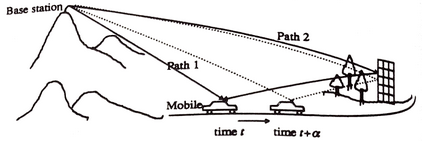
\includegraphics[width=\textwidth]{./Figures/%
		WirelessChannel/MultipathChannel.png}
	\caption{Multipath Channel \cite{Jer00}}
	\label{fig:MultipathChannel}
\end{figure} 

The resulting effect of this multipath channel is that %
symbols transmitted at different times will arrive %
at the receiver at the same time, this leads to %
a self-interfering effect that can cause the received %
signal power to undergo large fluctuations and can %
be characterised as inter-symbol interference.

The multipath fading can be broadly organised into %
two separate categories\cite{Jer00}.

\begin{enumerate}
	\item{The multipath signa paths are made up %
		of relatively small and identifiable number %
		of components reflected by small hills, %
		houses, and other strucutres encountered in %
		open areas and rural environments. This %
		results in a channel model with a finite number %
		of multipath components. Such a channel is %
		referred to as a \emph{discrete multipath channel}.}
	\item{The multipath signal paths are generated by %
		a large unresolvable reflections as might occur %
		in a mountainous area or in a dense urban environment. %
		This signal is composed of a continuum of %
		unresolvable multipath components. This %
		channel model is referred to as a \emph{diffuse %
		multipath channel}.}
\end{enumerate}

Small scale fading is caused by a transmitted signal %
arriving at the receiver with slightly different delays %
and angles after having been scattered or reflected by %
the environment in some way. The signals all self %
interfere at the receiver causing constructive or %
destructive interference. 

Multipath reflected components can be described in %
terms of orthogonal components $x_{n}(t)$ and %
$y_{n}$%
(t), where $x_{n}(t) + jy_{n}(t) = \alpha_{n}(t)e^{%
-j\theta_{n}(t)}$. If the number of random components %
is large enough and none are dominant, then the received %
components $x_{r}(t)$ and $y_{r}(t)$ which are the sums %
of the reflected signals will have a gaussian probability %
density function. The magnitude of the received scattered %
components will have a magnitude described by:

\begin{align}
	r_{0}(t) = \sqrt{x_{r}^{2}(t) + y_{r}^{2}(t)}
\end{align}

The probability density function of the envelope $r_{0}(t)$ %
of the received signal is going to follow a Rayleigh distribution %
with probability density function:

\begin{align}
	f_{R}(r) = \frac{r}{\sigma^{2}}e^{-r^{2}/(2\sigma^{2})}
	\label{eq:RayleighPDF}
\end{align}

\begin{figure}[h!]
	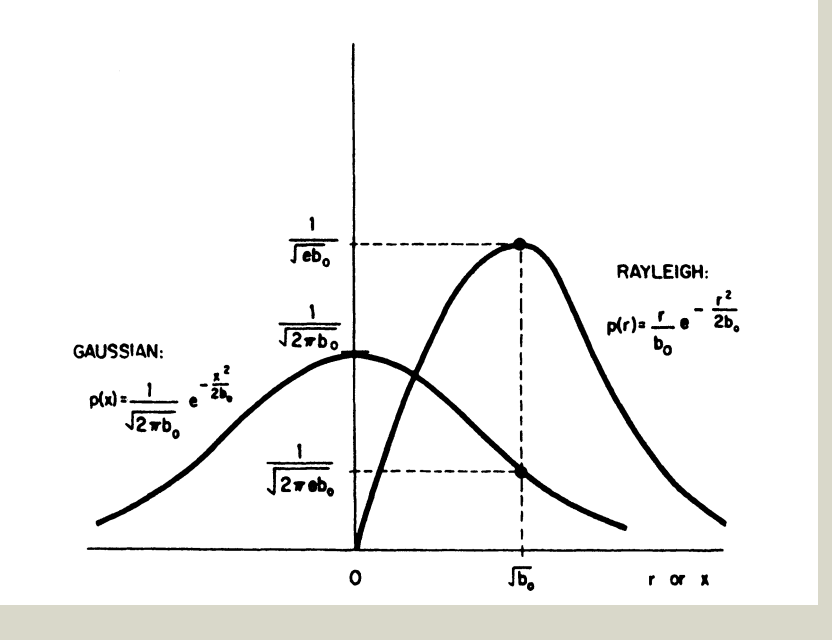
\includegraphics[width=\linewidth]{./Figures/%
	WirelessChannel/RayleighDistribution.png}
	\caption{Gaussian and Rayleigh Distributions%
	\cite{Jakes74}}
	\label{fig:RayleighDistribution}
\end{figure}

Figure \ref{fig:RayleighDistribution} illustrates %
the gaussian distribution and the rayleigh %
distribution.

When the received signal is made up of multiple %
reflected rays and a significant line-of-sight %
component, the received envelope ampliude %
follows a Rician distribution with probability density %
function:

\begin{align}
	f_{R}(r) = \frac{r}{\sigma^{2}}I_{0}%
	\left[ \frac{A_{r}}{\sigma^{2}} \right]%
	e^{-(r^{2}-A^{2})/(2 \sigma^{2})}
	\label{eq:RicianPDF}
	%I_{0} is the zeroth order modified bessel function
	% of the first kind
\end{align}

where $I_{0}$ is the modified zeroth order %
bessel function of the first kind. This kind of %
fading is commonly referred to as Rician fading. 
% Cite the text cited by Sklar???

% TODO: Explain the rician v parameter
% it comes from the expression describing the K parameter
\begin{figure}[h!]
	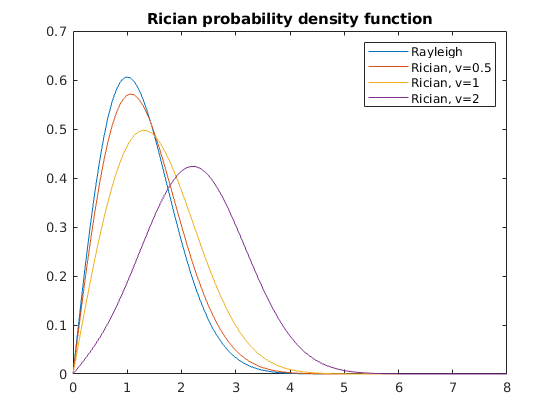
\includegraphics[width=\linewidth]{./Figures/%
	WirelessChannel/RicianDistribution.png}
	\caption{Rayleigh and Rician Distributions}
	\label{fig:RicianDistribution}
\end{figure}

% TODO: make a diagram of the Rician distribution
% TODO: find and plot a measured Rayleigh distribution



Good modeling and simulation of this small scale fading %
is crucial to the accurate simulation of wireless channels. %
There are two main methods of simulating small scale fading, %
the sums of sinusoids method first developed by Jakes in %
\cite{Jakes74} and a filtered white gaussian noise method. %
The filtered white gaussian noise methodology is the chosen %
method of simulation for this report.

\section{Wireless Channel as a Filter}

% TODO: Develop Finite impulse response filter model 
% of the wireless channel

% TODO: develop the model for the time-varying characteristics
% of wireless channels

% TODO: Develop the mathematics of the finite gaussian channel model


